\chapter{Einleitung}

Bei der Herstellung von integrierten Systemen und Schaltungen ist die Strukturierung der Proben im Nanometerbereich ein unumg�nglicher Prozesschritt. In der industriellen Fertigung hat sich die Fotolithografie etabliert. Mit ihr lassen sich vergleichsweise g�nstig und schnell Strukturen im Mikrometerbereich und kleiner herstellen. 

Sollen peridoische Strukturen hergestellt werden, bietet sich die Laserinterferenzlithographie an. So lassen sich mit dieser Technik z.B. Beugungsgitter mit hoher Genauigkeit und Linienbreiten von einigen hundert Nanometern herstellen. %So ist es m�glich Gitter mit Linienbreiten von einigen hundert Nanometern herzustellen. Das Verfahren wird zum Beispiel zur Herstellung von Reflektionsgittern, \textit{Grating Couplern}, oder zur Herstellung von Biosensoren verwendet. 
Weitere Anwendungsgebiete sind u.a. Gitterkoppler, \textit{Distributed Feedback Laser} oder Resonatoren z.B. f�r Biosensoren.

Im Labor Nanotechnologie am Lichttechnischen Institut (LTI) des KIT werden an einem Versuchstermin Gitterstrukturen mit der Laserinterferenzlithographie hergestellt. Es wird zum einen die Probenvorbereitung, die Belichtung und Entwicklung der Proben sowie Charakterisierung der selbst hergestellten Proben vorgenommen.

\chapter{Grundlagen und Versuchsaufbau}

Die Laserinterferenzlithographie nutzt den Effekt der Interferenz zweier Wellen. Hierzu wird koh�rentes, monochromatisches Licht aus einem Laser verwendet. Das Licht des Lasers wird mit einem Strahlteiler aufgeteilt. �ber Spiegel werden die Strahlen zur Probe hin umgelenkt und mit Linsen aufgeweitet um den Belichtungsbereich zu vergr��ern. Abbildung \ref{fig:aufbau}\footnote[1]{Uwe Bog; Laboratory Nanotechnology - Experiment: Laser Interference Lithography; Preperation Materials - Version 1.2}.  Veranschaulicht den beschriebenen Aufbau zur Laserinterferenzlithographie. Der verwendete Aufbau zur Probenherstellung beinhaltet einen Laser mit einer Wellenl�nge von $\lambda$~=~266~nm. Aufgrund der verwendeten Wellenl�nge im tiefen UV-bereich wurden die Linsen zur Strahlaufweitung im verwendeten Aufbau durch konkave Spiegel ersetzt. 

Beim Aufeinandertreffen der beiden Strahlen interagieren die elektromagnetischen Wellen beider Strahlen miteinander. Aufgrund von Phasenunterschieden beider Strahlen Addieren oder Subtrahieren sich die Amplituden beider Strahlen. Dies erzeugt ein sinusf�rmiges Interferenzmuster auf der Probenoberfl�che. 

Die Periode $P$ des sinusf�rmigen Interferenzmusters ist durch

\begin{figure}%
\centering
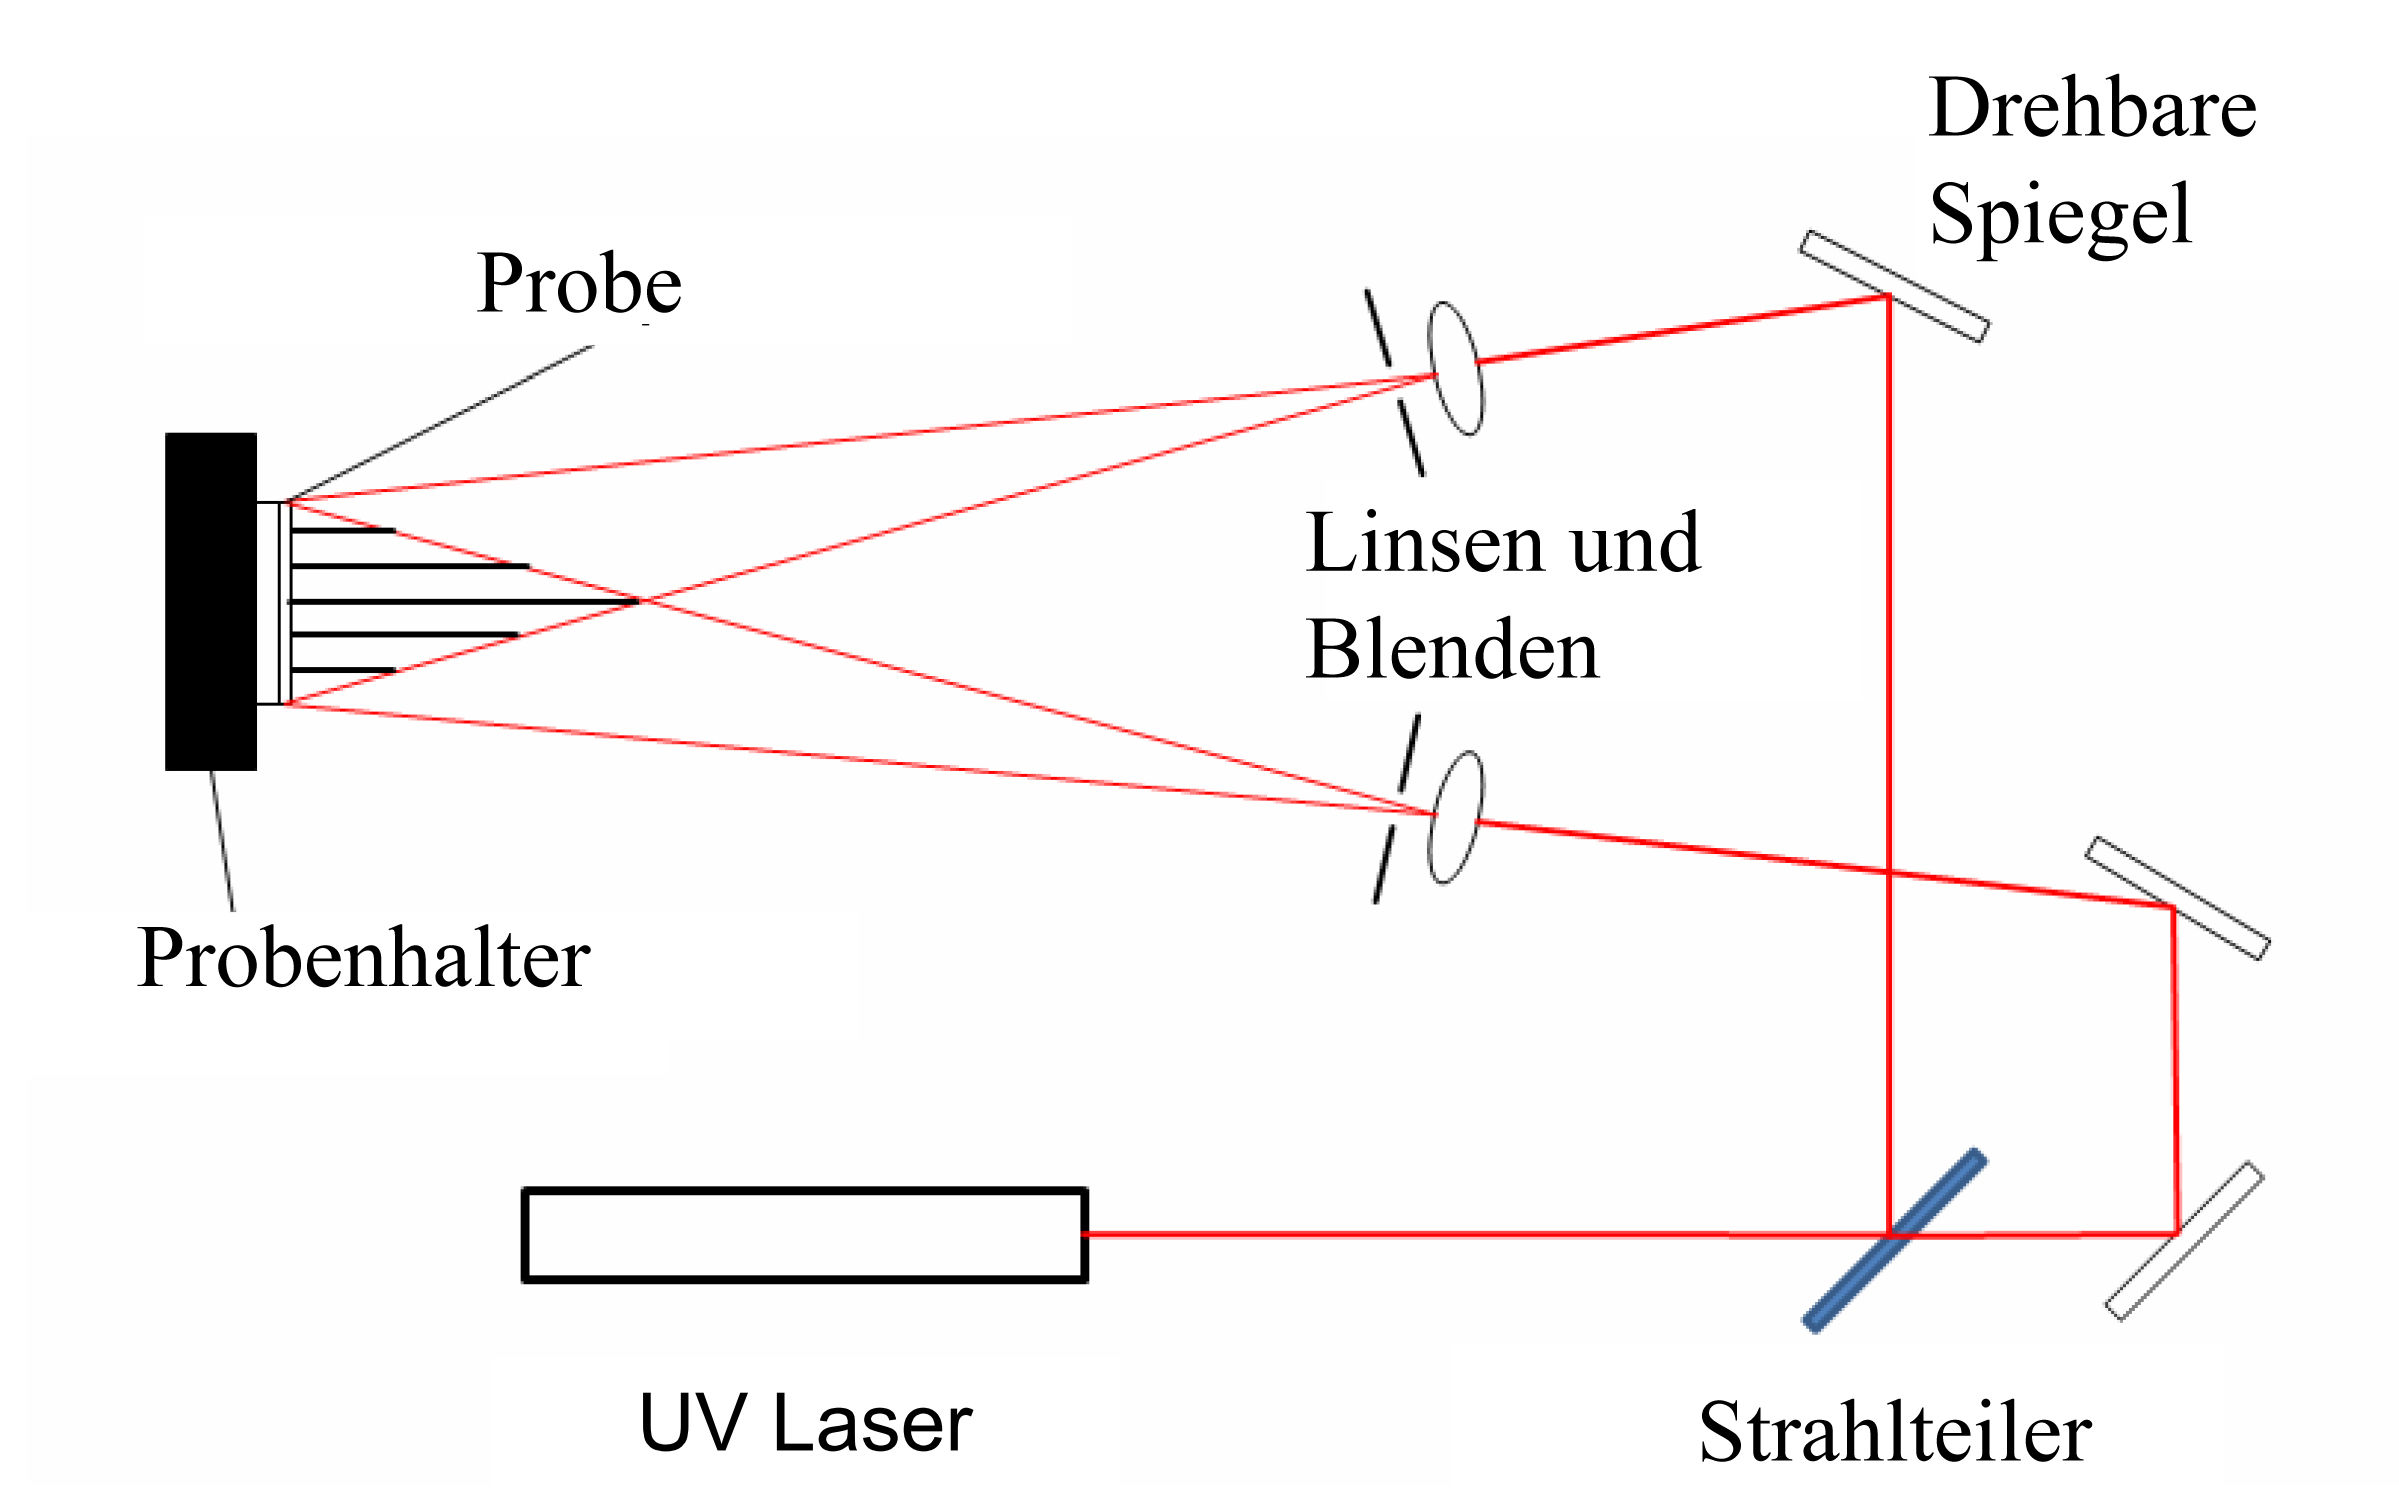
\includegraphics[width=.5\columnwidth]{Grafiken/aufbau.jpg}%
\caption{}%
\label{fig:aufbau}%
\end{figure}


\begin{equation}
P = \frac{\lambda}{2 n \cdot\mathrm{sin}\theta}
\label{eq:periode}
\end{equation}
gegeben. Hierbei ist $n$ die Brechzahl des �ber der Probe liegenden Mediums (z.B. Luft) \todo{Korrekt, dass ich hier Luft habe.. die in der Pr�sentation labern was vom Fotolack}, $\lambda$ die Wellenl�nge des verwendeten Lasers und $\theta$ der Winkel zur unter dem der Laserstrahl auf die Probe f�llt, gemessen zur Normalen zur Probe.

Auf der Probenoberfl�che ist ein Fotolack aufgebracht der durch das Interferenzmuster periodisch Belichtet wird. Die Wahl des verwendeten Fotolackes beeinflusst die hergestellten Strukturen ma�geblich. Ein Fotolack mit hohem Kontrast resultiert in einem Gitter mit steilen Kanten. Um eine flache sinusf�rmige Gitterstruktur herzustellen muss ein Fotolack mit geringem Kontrast verwendet werden.


\chapter{Versuchsdurchf�hrung}
Zun�chst wurde das Substrat f�r die Durchf�hrung des Versuches vorbereitet. Hierzu wurde das Glassubstrat zun�chst auf 25x25~mm$^2$ gro�e St�cke zurechtgeschnitten und mit Aceton und Isopropanol gereinigt. Um Feuchtigkeit aus dem Substrat zu verdr�ngen wurden die Proben f�r 10~min auf eine Hot-Plate mit 150~�C gelegt und anschlie�end in einem Plasmaverascher f�r 2~min einem Sauerstoffplasma ausgesetzt. Zur besseren Haftung des Lacks wurde dann per Vakuum-Sublimation eine Schicht Hexamethyldisilazan (HMDS) aufgetragen. Hierzu wurde ein Becherglas mit HMDS zusammen mit den Proben in einen Exsikkator gestellt. Durch das Evakuieren des Exsikkators verdampft nun das HMDS und lagert sich an der Oberfl�che des Substrats an.

Als n�chstes folgte das Auftragen des Fotolacks per Spin-Coating. Als Fotolack wurde der experimentelle Fotolack SX~AR-P~5300/4 verwendet. Das Spin-Coating erfolgte zun�chst f�r 5~s mit 500~min$^{-1}$ um den Lack gleichm�sig auf dem Substrat zu verteilen und anschlie�end f�r 45~s bei 4000~min$^{-1}$. Die hieraus resultierende Schichtdicke betr�gt ca. 1,5~$\upmu$m.
Schlie�lich wurden die Proben f�r 2~min auf eine Hotplate mit 110�C gelegt um das L�sungsmittel aus dem Fotolack auszutreiben.

Nun wurden die Proben in den LIL-Aufbau eingebaut und belichtet. Durch unterschiedliche Belichtungszeiten wurden Proben hergestellt, die mit unterschiedlichen Energien von 40, 80, 120 und 160~mJ belichtet wurden. Die Entwicklung der Proben wurde mit dem Entwickler AR 300-35 durchgef�hrt. Hierzu wurde dieser im Verh�ltnis 1:1 mit Wasser gemischt. In diese L�sung wurden die Proben anschlie�end getaucht und nach einer Entwicklungszeit von 2~s bis 10~s wieder herausgenommen und in ein Wasserbad getaucht um die Entwicklung zu stoppen. Zur �bersicht sind die bei der Herstellung variierten Parameter in Tabelle \ref{tab:parameter} zu sehen.

\begin{table}%
\centering
\caption{Herstellungsparameter der Proben}
\begin{tabular}{cc}

\toprule
Entwicklungsdauer	& Belichtungsenergien\\
in s	& in mJ\\
\midrule
2 & 40, 80\\
5  & 40, 80, 120, 160\\
10 & 80, 120, 160\\
\bottomrule 
\end{tabular}
\label{tab:parameter}
\end{table}
